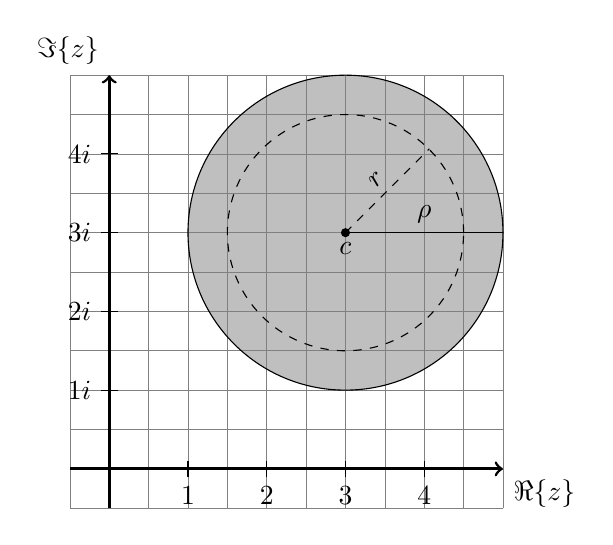
\begin{tikzpicture}
   % coords
   \coordinate (OR) at (0, 0);
   \coordinate (LX) at (-0.5, 0);
   \coordinate (RX) at (5, 0);
   \coordinate (TY) at (0, 5);
   \coordinate (BY) at (0, -0.5);

   % debugging grid
   \coordinate (BL) at (-0.5, -0.5);
   \coordinate (TR) at (5, 5);
   \draw[step=0.5cm, gray, very thin] (BL) grid (TR);

   % coordinate system
   \draw[->][line width=1.00pt] (LX) -- (RX) node[anchor=north west] {\(\Re\{z\}\)};
   \draw[->][line width=1.00pt] (BY) -- (TY) node[anchor=south east] {\(\Im\{z\}\)};
   \foreach \n in {1,2,...,4}{%
      \draw (\n,-3pt) node [below] {$\n$} -- (\n,3pt);
      \draw (-3pt,\n) node [left] {$\n i$} -- (3pt,\n);
   }

   \coordinate (c) at (3,3);
   \path[fill=gray, semitransparent] (c) circle (2);
   \draw[fill] (c) node[anchor=north]{\(c\)} circle [radius=0.05];
   \draw (c) circle (2);
   \draw (c) -- (5,3) node [midway, above, sloped, black] (TextNode) {\(\rho\)};

   \draw[dashed] (c) circle (1.5);
   \draw[dashed] (c) -- (4.065, 4.065) node [midway, above, sloped, black] (TextNode) {\(r\)};
\end{tikzpicture}
